\chapter{Design of the MagAO-X wavefront sensor}

\section{Introduction to Optical Design}

The basis of optical design is to design a system that meets given requirements and minimizes optical aberrations in the system. Optical designers use geometric optics to calculate the size and location of first order parameters in the optical system, which include the pupil planes, focal planes, stops, and nodal points. In geometric optics light is treated as a ray that is traced point to point through the optical system. The result is that one point in the image plane maps to one point in the object plane. It can model the effects of optical aberrations to calculate the error in ray propagation called optical path difference (OPD) for different ray heights and angles. Geometric optics cannot be used to predict the effects of the wave nature of light, such as diffraction and interferometry. 

Paraxial optics is a simplification to geometric optics that assumes the small angle approximation. It is a method for solving for the first order properties of a system using ray tracing equations. The paraxial approximation ignores the curvature of surfaces, but does take into account refraction through materials. The paraxial raytrace equations are,

\begin{eqnarray}
       n'u'=nu -y\phi  \label{4PWFSslopes} \\
       y'=y+u't' \nonumber \\
       \phi =(n'-n)C
\end{eqnarray}

where $n$ and $n'$ are the refractive index of the medium before and after propagation. The variables $u$ and $u'$, are the ray angles and $y$ and $y'$ are the ray heights. The distance between the starting point and the propagated point is $t'$. The variable $\phi$ is the power of a surface with curvature $C$ and refractive index $n'$. Figure \ref{fig:paraxial} shows an example setup of a raytrace,(\cite{greivenkamp2004field}). Various raytracing programs such as Zemax, CodeV, and Oslo implement paraxial raytracing modes to design optical systems. 


\begin{figure}
    \centering
    \includegraphics[width=.5\textwidth]{Chapter Materials/Chapter Three Materials/paraxialray.png}
    \caption{Setup for a paraxial ray trace. Starting point is from an object height $y$, with angle $u$. The ray is propagated a distance $t'$, until it hits a surface with power $\phi$, and refractive index $n'$. The ray height at this surface is $y'$, and exits with angle $u'$.}
    \label{fig:paraxial}
\end{figure}




Tracing the marginal and chief ray using the paraxial raytracing method determines important system parameters. The marginal ray has zero height at the object, passes through the maximum edge of the aperture stop, and is zero at the image plane. Tracing the marginal ray gives the positions of the object and image planes, and the height of the system stops. This includes the aperture stop, as well as the entrance and exit pupils of the system, which are the image of the aperture stop in the object and image planes respectively. The chief ray passes through the maximum edge of the object and image, and passes through the center of the aperture stop. It gives the object and image sizes as well as the location of the system stops. Figure \ref{fig:chiefray} shows an example ray trace of the marginal and chief ray through a lens with the stop at the lens. 


\begin{figure}
    \centering
    \includegraphics[width=.6\textwidth]{Chapter Materials/Chapter Three Materials/chiefandmarginal.png}
    \caption{Diagram of a ray trace for the marginal and cheif ray. The marginal ray starts at the optical axis at the location of the object, and is traced to the maximum edge of the system stop. It crosses the optical axis at the location of the image. The chief ray starts at the object height $h$, crosses the optical axis through the center of the stop, and intersects the maximum height of the image $h'$. }
    \label{fig:chiefray}
\end{figure}



Once the first order properties of the system are determined, the next step in the design process is to mitigate the optical aberrations that can be corrected for through design. A way to determine the aberrations in the system is to first trace the paraxial ray, and then trace a bundle of rays at different heights and angles of field to determine the deviation from the paraxial solution, which is the OPD. We describe these aberrations as coefficients in a power series. The wave aberration equations are useful because they allow us to calculate the wavefront error as a function of field, $H$, aperture vector, $\rho$, and the wavefront error coefficient for the associated aberration, $W_{ijk}$. The coordinate system for determining the wave aberrations is given in Figure \ref{fig:Seidel}. The generating function for the wave aberration polynomials is,


\begin{equation}
    W(H,\rho, \theta)=\sum_{ijk} W_{ijk} H^i \rho^j \cos^k\theta
\end{equation}

where $W(H,\rho, \theta)$ is the total wavefront error. We can use these polynomials to solve for ray aberrations $\epsilon$ which are the deviations from the paraxial image plane for the system in both the longitudinal (parallel to the optical axis), and transverse (perpendicular to the optical axis) directions. 

\begin{figure}
    \centering
    \includegraphics[width=.8\textwidth]{Chapter Materials/Chapter Three Materials/Seidelcoord.png}
    \caption{Coordinate system for the wave aberration polynomials. The field coordinate is given by $H$, and the location in the pupil plane is given by $\rho$. (FIGURE OUT HOW TO CITE CLASS NOTES THIS CAME FROM 503)}
    \label{fig:Seidel}
    \end{figure}
    
The first few aberrations can be mitigated by the optical design. The aberrations that are considered when designing a system are: defocus, tip/tilt, coma, astigmatism, spherical, field curvature, distortion, and chromatic aberration. These aberrations are first and third order abberations and the corresponding wave aberration equations that describe each aberration is found in Table \ref{tab:aberrations}. There are higher order variants of these polynomials, for example fifth-order astigmatism, but in general these terms are harder to correct and are compensated with first and third-order terms. Optical design programs have tools to help the designer reduce and balance the aberrations. Zemax OpticStudio outputs ray fan diagrams that describe the total OPD amplitude and shape as a function of $\rho$. Individual Seidel coefficients for specific aberrations can be minimized through the system optimization Merit function. Different weights in the merit function can prioritize the correction of one aberration over others. 


\begin{table}
	\begin{center}
		\begin{tabular}{ | l| l | }
			\hline
			\textbf{Aberration}& \textbf{Wave Aberration Equation} \\ \hline
			Defocus & $W_{020}\rho^2$\\ \hline
			Tip/Tilt & $W_{111}H\rho \cos\theta$ \\ \hline
			Coma & $W_{131}H\rho^3\cos\theta$  \\ \hline
			Astigmatism & $W_{222}H^2\rho^2\cos^2\theta$  \\ \hline
			Spherical Aberration & $W_{040}\rho^4$ \\ \hline
			Field Curvature & $W_{220}H^2\rho^2$ \\ \hline
			Distortion & $W_{311}H^3 \rho \cos\theta$ \\ \hline
				
		\end{tabular}
	\end{center}
	\caption{Caption}
	\label{tab:aberrations}
\end{table}

In free space optical design it is common to work with spherical lenses because they are easy to manufacture. These lenses can introduce significant spherical and chromatic aberrations into the optical system. In this section we will briefly describe these aberrations, and how to mitigate them through design.  

\subsection{Spherical Aberration}

Spherical aberration is defined as the variation of focus by position of the aperture. It is caused by spherical surfaces, and in lenses it is due to the variation of thickness of the glass as a function of aperture due to the curvature of the lens surfaces. For a converging lens the effect is that rays that intersect near the edges of the lens aperture are bent more, and come to a focus before the rays that pass closer to the center. This effect is shown in Figure \ref{fig:spherical}. 

\begin{figure}
    \centering
    \includegraphics[width=.8\textwidth]{Chapter Materials/Chapter Three Materials/spherical.png}
    \caption{Diagram of rays incident on a plano-convex lens. The effect of spherical aberration can be seen by rays that are closer to the edges of the lens coming to a focus before those that are closer to the center of the lens. }
    \label{fig:spherical}
\end{figure}

There are a number of ways spherical aberration can be minimized in an optical system. The simplest method is to balance spherical aberration with defocus. This method is not ideal because there can be significant residual wavefront error. For custom lens design splitting the lens into a doublet ] to lessen the curvature of the surfaces reduces third spherical aberration by about a third or a fourth. Changing the shape factor of the lens changes the curvature and thickness of the lens while maintaining focal length. The shape factor is a measure of overall curvature of a lens and is calculated using,

\begin{equation}
    X=\frac{C_1-C_2}{C_1+C_2}
\end{equation}
where $C_1$ and $C_2$ are the front and back curvatures of the lens. Lenses with high shape factors have extreme curvatures and large spherical aberrations. Figure \ref{fig:shapefactor} compares lenses with the same focal lengths with high shape factor (A), and low shape factor (B). Making a surface of the lens aspheric or introducing an aspheric corrector plate can be used to illuminate or correct spherical aberration. Aspheric surfaces are harder to manufacture and increase system cost and complexity. Aberrations scale with the index of refraction. Using a lens made of a glass with high refractive index reduces spherical aberrations. There are other tricks for reducing spherical aberrations such as exploiting stop locations, that are more system specific and might not be applicable to all optical designs. 

\begin{figure}
    \centering
    \includegraphics[width=.8\textwidth]{Chapter Materials/Chapter Three Materials/ShapeFactor.png}
    \caption{ Diagram of the effect of shape factor on the amount of spherical aberration of lens made in Zemax. A. This lens has a shape factor 5 and exhibits strong spherical aberration due to the extreme curvature of the lens surfaces. B. Lens with a shape factor 1. Spherical aberration is minimized.}
    \label{fig:shapefactor}
\end{figure}


\subsection{Chromatic Aberrations}

Chromatic aberration is caused by the wavelength dependence of the index of refraction, which causes the refracted angle of a light ray to change according to wavelength. The effect of longitudinal chromatic aberration is that different wavelengths come to a focus at different points on the optical axis. Lateral chromatic aberration causes a variation in image magnification as a function of wavelength. We measure the amount of chromatic aberration with respect to different Fraunhofer absorption lines; the F line at $\lambda_F=486.1 nm$, the D line at $\lambda_D=589.2 nm$, and the C line at $\lambda_C= 656.3 nm$. The chromatic focal shift, $\delta_{FC}$,  is given calculated with respect to the $F$ and $C$ lines and is given by,

\begin{equation}
    \delta_{FC}=\frac{\phi_F-\phi_C}{\phi_F \phi_C}
\end{equation}


where $\phi$ is the optical power of the lens at those wavelengths. In optical design we measure the chromatic focal shift as a function of wavelength. Figure \ref{fig:focalshift} shows the chromatic focal shift of a singlet lens made of BK-7 glass.

\begin{figure}
    \centering
    \includegraphics[width=.7\textwidth]{Chapter Materials/Chapter Three Materials/focalshift.png}
    \caption{Diagram of the chromatic focal shift of a singlet lens made of BK-7 glass. The shift in focal length due to chromatic aberration is plotted agains wavelength.}
    \label{fig:focalshift}
\end{figure}

To correct for chromatic aberration we try and balance the chromatic focal shift by constructing a lens that places two or more wavelengths at the same focal length. For a single lens system we compensate the chromatic error by constructing achromatic doublets and triplets. An achromatic doublet is a pair of lenses, usually one positive lens and one negative lens, made of different materials that form a single lens. These lenses can be air spaced or cemented together. The crown glass is usually used for the positive lens, and the flint glass for the negative lens. An example of a crown-flint achromatic doublet designed in Zemax is shown in Figure \ref{fig:crownflint}.

\begin{figure}
    \centering
    \includegraphics[width=.8\textwidth]{Chapter Materials/Chapter Three Materials/doublet.jpg}
    \caption{Diagram of an achromatic doublet. The first lens is a positive lens made of crown glass. The negative lens is made from flint glass. }
    \label{fig:crownflint}
\end{figure}

The Abbe number, $\nu_d$, of a glass quantifies the material's dispersion. It is calculated by the using the refractive index of the material ad the F,D, and C lines. The equation for Abbe number is given in Equation \ref{abbe}. 

\begin{equation}
    \nu_d=\frac{n_D-1}{n_F-n_C}
    \label{abbe}
\end{equation}

Low Abbe numbers correspond to high dispersion. One of the lenses in the doublet is made from a type of glass called a crown glass that has a low refractive index, and low dispersion. The other lens is made of a flint glass, which has a high refractive index and a high dispersion. The combination of the two glass types corrects for chromatic aberrations by shifting the F and C focal lengths close together. In general this is best achieved when there is a large difference in the Abbe numbers of the glasses. The system of equations used to solve for the power of each lens is,
%
\begin{eqnarray}
       \delta \phi_{FC}=\phi_F-\phi_C=0 \\
       \frac{\phi_{1}}{\phi_T}= \frac{\nu_1}{\nu_1-\nu_2} \\
       \frac{\phi_{2}}{\phi_T}= \frac{-\nu_2}{\nu_1-\nu_2}\nonumber
\end{eqnarray}
where $\phi_T$ is the total system power, and $\phi_1$ and $\phi_2$ are the the power of each lens at the D wavelength. Figure \ref{fig:doublet} shows an example chromatic focal shift diagram created by an achromatic doublet made from BK-7 and F4 glass. 

\begin{figure}
    \centering
    \includegraphics[width=.8\textwidth]{Chapter Materials/Chapter Three Materials/doubletfocalshift.png}
    \caption{Focal shift diagram of an achromatic doublet from BK-7 and F4 glass. Achromatic doublets balance chromatic aberration by setting the focal shift of two different wavelengths in the bandpass to 0.}
    \label{fig:doublet}
\end{figure}

Achromatic triplets correct for both chromatic aberration and secondary chromatic aberration. Secondary chromatic aberration, or secondary spectrum, is caused by the third D wavelength coming to focus at a different spot than the focal shift corrected F and C wavelengths. Minimizing the focal shift between all three wavelengths is the method of correcting for secondary spectrum. Secondary chromatic aberration is compensated by considering the dispersion $P$ of a material, given by Equation \ref{dispersion}. The secondary chromatic aberration is controlled by choosing glasses that have very similar dispersion, but a large difference in Abbe number. 

\begin{equation}
    P=\frac{n_d-n_c}{n_F-n_C}
    \label{dispersion}
\end{equation}



A apochromatic lens is a triplet lens that balances the chromatic focal shifts and secondary chromatic aberrations at three wavelengths. The system of equations for the apochromatic triplet is,


\begin{eqnarray}
       \phi_1=\frac{(P_2-P_3)\nu_1}{(P_2-P_1)E}\phi_T \\
       \phi_2=\frac{(P_3-P_1)\nu_2}{(P_2-P_1)E}\phi_T \\
       \phi_3=\frac{(P_1-P_2)\nu_3}{(P_2-P_1)E}\phi_T \\
       E=\frac{(P_2-P_3)\nu_1+(P_3-P_1)\nu_2}{(P_2-P_1)}-\nu_3
\end{eqnarray}
where $P_1$,$P_2$, and $P_3$ are the dispersion's of each of the lenses in the triplet. The solution to these equations is that glass 1 and 3 should have very different dispersions and Abbe numbers to minimize chromatic aberrations, and that the second glass should have a $P$ and $\nu$ value that falls in between roughly halfway between the two. This is best visualized in Figure \ref{fig:tripletPV}, which plots the dispersion vs Abbe number for the different glass types in a triplet. 
\begin{figure}
    \centering
    \includegraphics[width=.6\textwidth]{Chapter Materials/Chapter Three Materials/tripletPV.png}
    \caption{Dispersion $P$ versus Abbe number $\nu_d$ for an achromatic triplet made from N-PK51, N-KZFS4, and N-SF15 glass types, (\cite{kingslake2009lens}).} 
    \label{fig:tripletPV}
\end{figure}

The resulting chromatic focal shift diagram for a triplet lens has three zero points as shown in Figure \ref{fig:apochromat} for a 100mm focal length apochromatic triplet made of N-LLF1,N-LAF33, and N-BK7 glass types by \cite{sasian2017method}. 

\begin{figure}
    \centering
    \includegraphics[width=.6\textwidth]{Chapter Materials/Chapter Three Materials/tripleapochromat.PNG}
    \caption{Chromatic focal shift diagram for an apochromatic triplet lens. The first and secondary chromatic aberrations are compensated in the lens creating three wavelengths where a zero chromatic focal shift occurs,(\cite{sasian2017method}).}
    \label{fig:apochromat}
\end{figure}









\section{MagAO-X}
	
the University of Arizona Extreme Wavefront Control Lab (XWCL), has developed the Magellan Extreme Adaptive Optics system (MagAO-X) for the Magellan Clay Telescope at Las Campanas Observatory, Chile,(\cite{males2020magao}). MagAO-X had its first light commissioning run in 2019b. The MagAO-X system uses a combination of a 2048 actuator deformable mirror, high speed pyramid wavefront sensor, and high contrast coronagraph to correct for atmospheric turbulence and suppress starlight at speeds greater than 2000 times a second. The instrument is designed to achieve Strehl ratios of greater than 70$\%$ with raw contrast of less than $10^{-4}$ at separations between 1 and 10 $\lambda/D$.\cite{males2018magao} Working off of lessons learned from MagAO ,(\cite{close2018status}), and SCExAO, (\cite{jovanovic2015subaru}), MagAO-X is optimized for high impact science cases, such as a survey of nearby newly formed acretting planets in H$\alpha$, (\cite{males2020magao}).

The MagAO-X system has a two-level split optical table, mounted at the gravity invariant Nasymth platform. The table is floated to reduce vibrations, and sealed in dust covers to shield against dust and stray light. The top optical table contains the K-mirror, (\cite{hedglen2018optical}), the low order ALPAO DM97 woofer deformable mirror, the high order tweeter BMC-2K deformable mirror, and the atmospheric dispersion corrector (ADC). The lower bench contains another ALPAO DM97 DM to correct non common path errors in the coronagraphs. There are two Princeton science camera to enable spectral differential imaging, (\cite{biller_sdi}). MagAO-X has a generalized Lyot coronagraph with a vector Apodizing Phase Plate (vAPP) mask. A four-sided pyramid PWFS provides the high order wavefront sensing. Figure REF shows the layout of the MagAO-X system. In this chapter we will describe the optical design of the MagAO-X pyramid wavefront sensor and the requirements on performance that drove the design choices. 

MAGAO-X FIGURE CHECK THE BOX

\section{System Design}

The PWFS of the MagAO-X system consists of an achromatic pyramid, a camera lens, and an OCAM$^2$K EMCCD detector. The requirements on the MagAO-X PWFS were a needed size and separation of the pupils, and a restricted system size to fit on the optical table. The MagAO-X pyramid wavefront sensor is designed to operate from 600-1000nm bandwidth and a field of view of two arcseconds. Figure \ref{fig:bandpass} is the bandpass of the MagAO PWFS that we matched for the MagAO-X PWFS. A new camera lens was designed in Zemax to meet the requirements of the MagAO-X system. 
	
	
\begin{figure}[h]
	\centering
	\includegraphics[width=.5\textwidth]{Chapter Materials/Chapter Three Materials/MagAOBandpass_updated.jpg}
	\caption{Transmission versus wavelength for the V, R, and I bandpasses. The overlaid black curve is MagAO-X pyramid wavefront sensor bandpass that is matched from MagAO,(\cite{morzinski2014magao}).}
	\label{fig:bandpass}
\end{figure}
	
 The requirements of the MagAO-X PWFS are listed in Table \ref{tab:requirements}. The OCAM$^2$K is used in the 2x2 binning mode, which gives and effective pixel size of 48 $\mu$m. This allows the wavefront sensor to be run at speeds up to 3.6 kHz. The pupil size is 56 pixels in diameter. The number of pixels in each of the pupils sets the sampling of the wavefront which determines the number of modes correctable by the AO system and the fitting error in the AO error budget. This sampling was chosen to meet the performance goals of the MagAO-X wavefront control. The pupil separation of 60 pixels was chosen to maximize space on the OCAM$^2$K detector. Figure \ref{fig:PWFSpupils} summarizes the desired layout for the PWFS pupils on the OCAM$^2$K detector. 
	
\begin{table}
	\begin{center}
		\begin{tabular}{ | l| l | }
			\hline
			\textbf{Parameter}& \textbf{Requirement} \\ \hline
			Wavelength Range &600- 1000 nm \\ \hline
			Pupil Size & 56 pixels; 2.688 mm \\ \hline
			Pupil Separation & 60 pixels; 2.880 mm  \\ \hline
			Pupil Tolerances & $\Delta$ $<$ 1/10th pixel; 2.4 $\mu$m  \\ \hline
			Lens Diameter & 10 mm $<$ D  $<$ 20 mm \\ \hline
				
		\end{tabular}
	\end{center}
	\caption{Parameters and their requirements for the MagAO-X pyramid wavefront sensor.}
	\label{tab:requirements}
\end{table}

\begin{figure}
    \centering
    \includegraphics[width=.5\textwidth]{Chapter Materials/Chapter Three Materials/MagAOXpupils.png}
    \caption{Diagram of the desired pupil layout on the OCAM$2$K detector produced by the PWFS. The pupils fall on a gril of 128 by 128 pixels, each pixel having a size of 48 $\mu m$. Each pupil is designed have a diameter of 56 pixels across, and seperated by 60 pixels center to center.}
    \label{fig:PWFSpupils}
\end{figure}
    
The tolerance on the pupil sizes is 1/10$^{th}$ of a pixel, which is 2.4 $\mu m$. Due to the tight tolerances on pupil size, and the large bandpass of the system a custom achromatic triplet lens was designed as the camera lens for the MagAO-X PWFS. The triplet lens allows for the minimization of spherical aberration by allowing for the reduction in curvature of each lens in the triplet, while maintaining the effective focal length needed to meet the magnification requirements. Transverse spherical aberration, which causes a difference in magnification as function of aperture is important to mitigate in this system, because the size of each pupil needs to be uniform. Similarly, lateral chromatic aberration needs to be controlled, because the size of the pupils cannot vary over the bandpass.
	
	
\subsection{Pyramid Design}
MagAO-X will uses an excellent achromatic pyramid with a 5 $\mu m$ tip. The pyramid used in the PWFS is a double pyramid, consisting of two four sided prisms aligned back to back. Details of the design done by \cite{tozzi2008double} are summarized here. A picture of the pyramid is shown in Figure \ref{fig:pyramid}. The total deviation angle needed for the pyramid wavefront sensor is hard to manufacture. Combining two pyramids makes the polishing process easier and at the same time allows us to control chromatic aberrations by using two different glass types. The glass types were chosen using an I.D.L. optimization routine that selected glass combinations from the Shott and Ohara catalog that would give a suitable deflection angle of the double pyramid. The front prism is made from Shott N-SK11, $n_d=1.56384$ and $\nu_D=60.80$, and the back prism is made from Schott N-PSK53, $n_d=1.61800$ and $\nu_D=63.39$. The full diagram of the achromatic double pyramid is found in Figure \ref{fig:fullpyramidprism}.




	
\begin{figure}[h]
	\centering
	\includegraphics[width=.5\textwidth]{Chapter Materials/Chapter Three Materials/pyramid.png}
	\caption{Fabricated pyramid made in Arcetri, Italy by Paolo Stefanini.}
	\label{fig:pyramidprism}
\end{figure}
	
\begin{figure}
    \centering
    \includegraphics[width=.6\textwidth]{Chapter Materials/Chapter Three Materials/pyramidprismfull.JPG}
    \caption{Drawing of the optical design of the MagAO-X achromatic double pyramid. The pyramid has a high precision entrance pyramid (in blue) made of N-SK11 glass. The exit pyramid (in red) is made of N-PSK53 glass. The angles of the pyramid are designed so that the total deviation of the pair is small.}
    \label{fig:fullpyramidprism}
\end{figure}
	
	
	
\subsection{Wavefront Sensor Design}
	
A design of the wavefront sensor was done in Zemax OpticStudio. An F/69 beam created by an off-axis parabolic (OAP) mirror is focused onto the pyramid tip. A custom achromatic triplet then images four pupils onto our OCAM$^2$K wavefront sensor camera. A layout of the wavefront sensor optical path done in both Zemax and SolidWorks is shown in Figure \ref{fig:oplayout}. We reuse the same off axis parabolic mirror seen by the coronagraph arm of MagAO-X. The double pyramid was modeled by the Arcetri team, (\cite{tozzi2008double}). A custom achromatic triplet was designed to give the correct pupil size and separation. The two windows in the OCAM$^2$K detector are included in the design for completeness. The expected pupil footprint on the image plane for 800 nm wavelength is given in Figure \ref{fig:footprint}. Restraints were placed in the merit function to limit the path length of the PWFS. 

\begin{figure}[h]
	\centering
	\includegraphics[width=.5\textwidth]{Chapter Materials/Chapter Three Materials/Pupils6-20-18.jpg}
	\caption{Beam footprint diagram at the image plane. Each colored circle is a pupil.}
	\label{fig:footprint}
\end{figure}

\begin{figure}
    \centering
    \includegraphics[width=.8\textwidth]{Chapter Materials/Chapter Three Materials/layout.jpg}
    \caption{Optical path of the PWFS in Zemax. The 5$^{th}$ OAP mirror forms an F/69 focus on the tip of the double pyramid. The triplet camera lens images the pupils onto the OCAM$^2$K camera.}
    \label{fig:my_label}
\end{figure}

\begin{figure}
    \centering
    \includegraphics[width=.8\textwidth]{Chapter Materials/Chapter Three Materials/PWFSOptoMech.jpg}
    \caption{Layout of the pyramid wavefront sensor (green path) on the MagAO-X optical bench, (\cite{close2018optical}). The Zemax ray trace was imported into SolidWorks for the optomechanical design. The red-light path is the science path that goes to the coronagraph.}
    \label{fig:oplayout}
\end{figure}
	
	
	
	
\subsection{Achromatic Triplet Design}

The size and separation of the pupils on the detector directly affects the performance of the PWFS. If the pupils are undersized, there will be aliasing in reconstruction of the higher order modes. If the separation between pupils is not correct, complications will arise when pixels are binned on the detector to change the pupil sampling and the integration time.  To ensure the correct size and separations a custom achromatic triplet was designed in Zemax. A schematic of the lens is shown in Figure \ref{fig:triplet}. 


\begin{figure}[h]
	\centering
	\includegraphics[width=.8\textwidth]{Chapter Materials/Chapter Three Materials/cameralenstripletSPEC.jpg}
	\caption{Lens schematic of the achromatic triplet in zemax. The radius of curvatures of each surface are listed under the Radius column. The material and thickness of each lens is given in under Material and Thick columns.  }
	\label{fig:triplet}
\end{figure}


In the optimization merit function restraints were place to insure that the triplet was manufacturable, and met our system requirements. The thickness at the middle and edges of each of the lenses in the triplet were constrained to insure that the lens was of reasonable curvature and the system did not converge to an impossible shape. The main focus of the merit function was to insure that the pupil sizes and separations were the same as a function of field and wavelength. This was done by calculating coordinates of the edges of the pupils using real ray tracing operands, and then using math operands to use the coordinates to calculate pupil size and spacing. Targets for the size and spacing were then set to the desired values, and a large weight was applied to each of these operands to force the system to converge to our desired outcome.


%%%%% Go in and show a photo of the merit function?
	
A tolerance analysis to determine lens performance as a function of wavelength is done using parameters from the Precision grade Optimax manufacturing tolerancing chart. Reasonable values of alignment errors were estimated and included in the tolerancing analysis. The figure of merit used was the RMS angular radius of the lens because the pyramid is an afocal system. A 500 trial Monte Carlo simulation was done for three wavelengths, 600nm, 800nm, and 1000nm. At each wavelength the nominal, mean, and worst RMS angular size (twice the angular radius) was recorded. The difference of the mean and worst angles with respect to the nominal value was calculated. That change in angle was propagated through the system to estimate the change in size we would expect. The propagation is shown in Figure \ref{fig:propagation}, where $\theta_n$ is the nominal RMS angular size, and $\theta_\Delta$ is the change in RMS angular size we use to calculate the estimated change $\Delta y$. The distances $x_1 ... x_5$ were taken from the Zemax design, and the indexes $n_1, n_2, n_3$ correspond to air, BK-7, and Sapphire respectively. The index of refraction was adjusted for the different wavelengths when the propagation was calculated using trigonometry and Snell's law. The results are summarized in Figure \ref{fig:change}, where the change in size in nanometers is graphed against wavelength. At worst we expect about a 45 nm change in pupil size and separation, but no change on average. Both are well within our tolerance of the change being no greater than 1/10th a pixel, or 2.4$\mu$m.
	
	
	
\begin{figure}[h]
	\centering
	\includegraphics[width=.8\textwidth]{Chapter Materials/Chapter Three Materials/propagation.JPG}
	\caption{Diagram of the light propagation path used to calculate the change in pupil size. Light is propogated from surface to surface using paraxial ray tracing and Snell's law.}
	\label{fig:propagation}
\end{figure}
	
	
\begin{figure}[h]
	\centering
	\includegraphics[width=.5\textwidth]{Chapter Materials/Chapter Three Materials/achromaticchangegraph.jpg}
	\caption{Expected change in pupil size as a function of wavelength.}
	\label{fig:change}
\end{figure}
	
\section{System Performance}
	
A simulation of the expected partial illumination of pupil pixels was done in MATLAB. A binary model of the MagAO-X pupil was generated with 10 times the spatial sampling than our expected PWFS pupil. We then bin it down to the expected pupil sampling of our PWFS. That is, we start with a pupil of 560 by 560 pixels, and bin down to a 56 by 56 pixel pupil by summing 10 by 10 pixel bins and normalizing. The expected illumination pattern is shown in Figure \ref{fig: pupilpixels}. A table of the pixel counts is given in Table \ref{tab:actuators}. We expect 1958 fully illuminated pixels within our pupil. 
	
	
\begin{figure}%
	\centering
	\includegraphics[width=.4\textwidth]{Chapter Materials/Chapter Three Materials/pupilpixels.jpg}
	\caption{Expected pupil illumination on the PWFS.}	
	\label{fig: pupilpixels}
\end{figure}
	
	
	
\begin{table}[h]
	\begin{center}       
		\begin{tabular}{|l|l|} %% this creates two columns
				%% |l|l| to left justify each column entry
				%% |c|c| to center each column entry
				
				\hline%% use of \rule[]{}{} below opens up each row
				\rule[-1ex]{0pt}{3.5ex} $\%$ \textbf{Illumination} & \textbf{$\#$ of Pixels }  \\
				
				\hline%% use of \rule[]{}{} below opens up each row
				\rule[-1ex]{0pt}{3.5ex} 100$\%$ & 1958  \\
				\hline%% use of \rule[]{}{} below opens up each row
				\rule[-1ex]{0pt}{3.5ex} 90$\%$ & 166  \\
				\hline%% use of \rule[]{}{} below opens up each row
				\rule[-1ex]{0pt}{3.5ex} 80$\%$ & 24  \\
				\hline%% use of \rule[]{}{} below opens up each row
				\rule[-1ex]{0pt}{3.5ex} 0$\%$ & 46  \\
				\hline%% use of \rule[]{}{} below opens up each row
				\rule[-1ex]{0pt}{3.5ex} 60$\%$ & 20  \\
				\hline%% use of \rule[]{}{} below opens up each row
				\rule[-1ex]{0pt}{3.5ex} 50$\%$ & 18  \\
				\hline%% use of \rule[]{}{} below opens up each row
				\rule[-1ex]{0pt}{3.5ex} $<$ 50$\%$ & 904  \\
				\hline
		\end{tabular}
	\end{center}
	\caption{Percentage of illuminated pixels one of the 56 by 56 pixel pupils. }
	\label{tab:actuators}
\end{table}
	
\section{Initial Results}
	
The camera triplet was manufactured by Rainbow optics and the as-built specifications of the lens was incorporated into the Zemax design. The tolerance of our system was that the pupil size and separation would be within 1/10$^{th}$ of a pixel. We found that our fabricated lens was slightly under specifications. The pupils are slightly oversized, and the pupil separation is too close together. Table \ref{tab:asbuilt} shows the system requirements of the MagAO-X system, and the expected performance with our fabricated lens. The lens was mounted in a piezo-motorized stage shown in Figure, that allowed for X-Y positioning, as well as rotation. 
	
	
\begin{table}
	\begin{center}
		\begin{tabular}{ | l| l |  l |}
			\hline
			\textbf{Parameter}& \textbf{Requirement} & \textbf{As Built}\\ \hline
			Wavelength Range &600- 1000 nm& 600-1000 nm\\ \hline
			Pupil Size & 56 pixels; 2.688 mm& 2.696 mm\\ \hline
			Pupil Separation & 60 pixels; 2.880 mm& 2.857 mm \\ \hline
			Pupil Tolerances & $\Delta$ $<$ 1/10th pixel; 2.4 $\mu$m& $\Delta_{size}$=8 $\mu m$,  $\Delta_{sep}$=-23 $\mu m$ \\ \hline
			Lens Diameter & 10 mm $<$ D  $<$ 20 mm & D= 10.1 mm\\ \hline
				
		\end{tabular}
	\end{center}
	\caption{Parameters for the MagAO-X pyramid wavefront sensor and the as built expected performance from our Zemax model.}
	\label{tab:asbuilt}
\end{table}



\begin{figure}
    \centering
    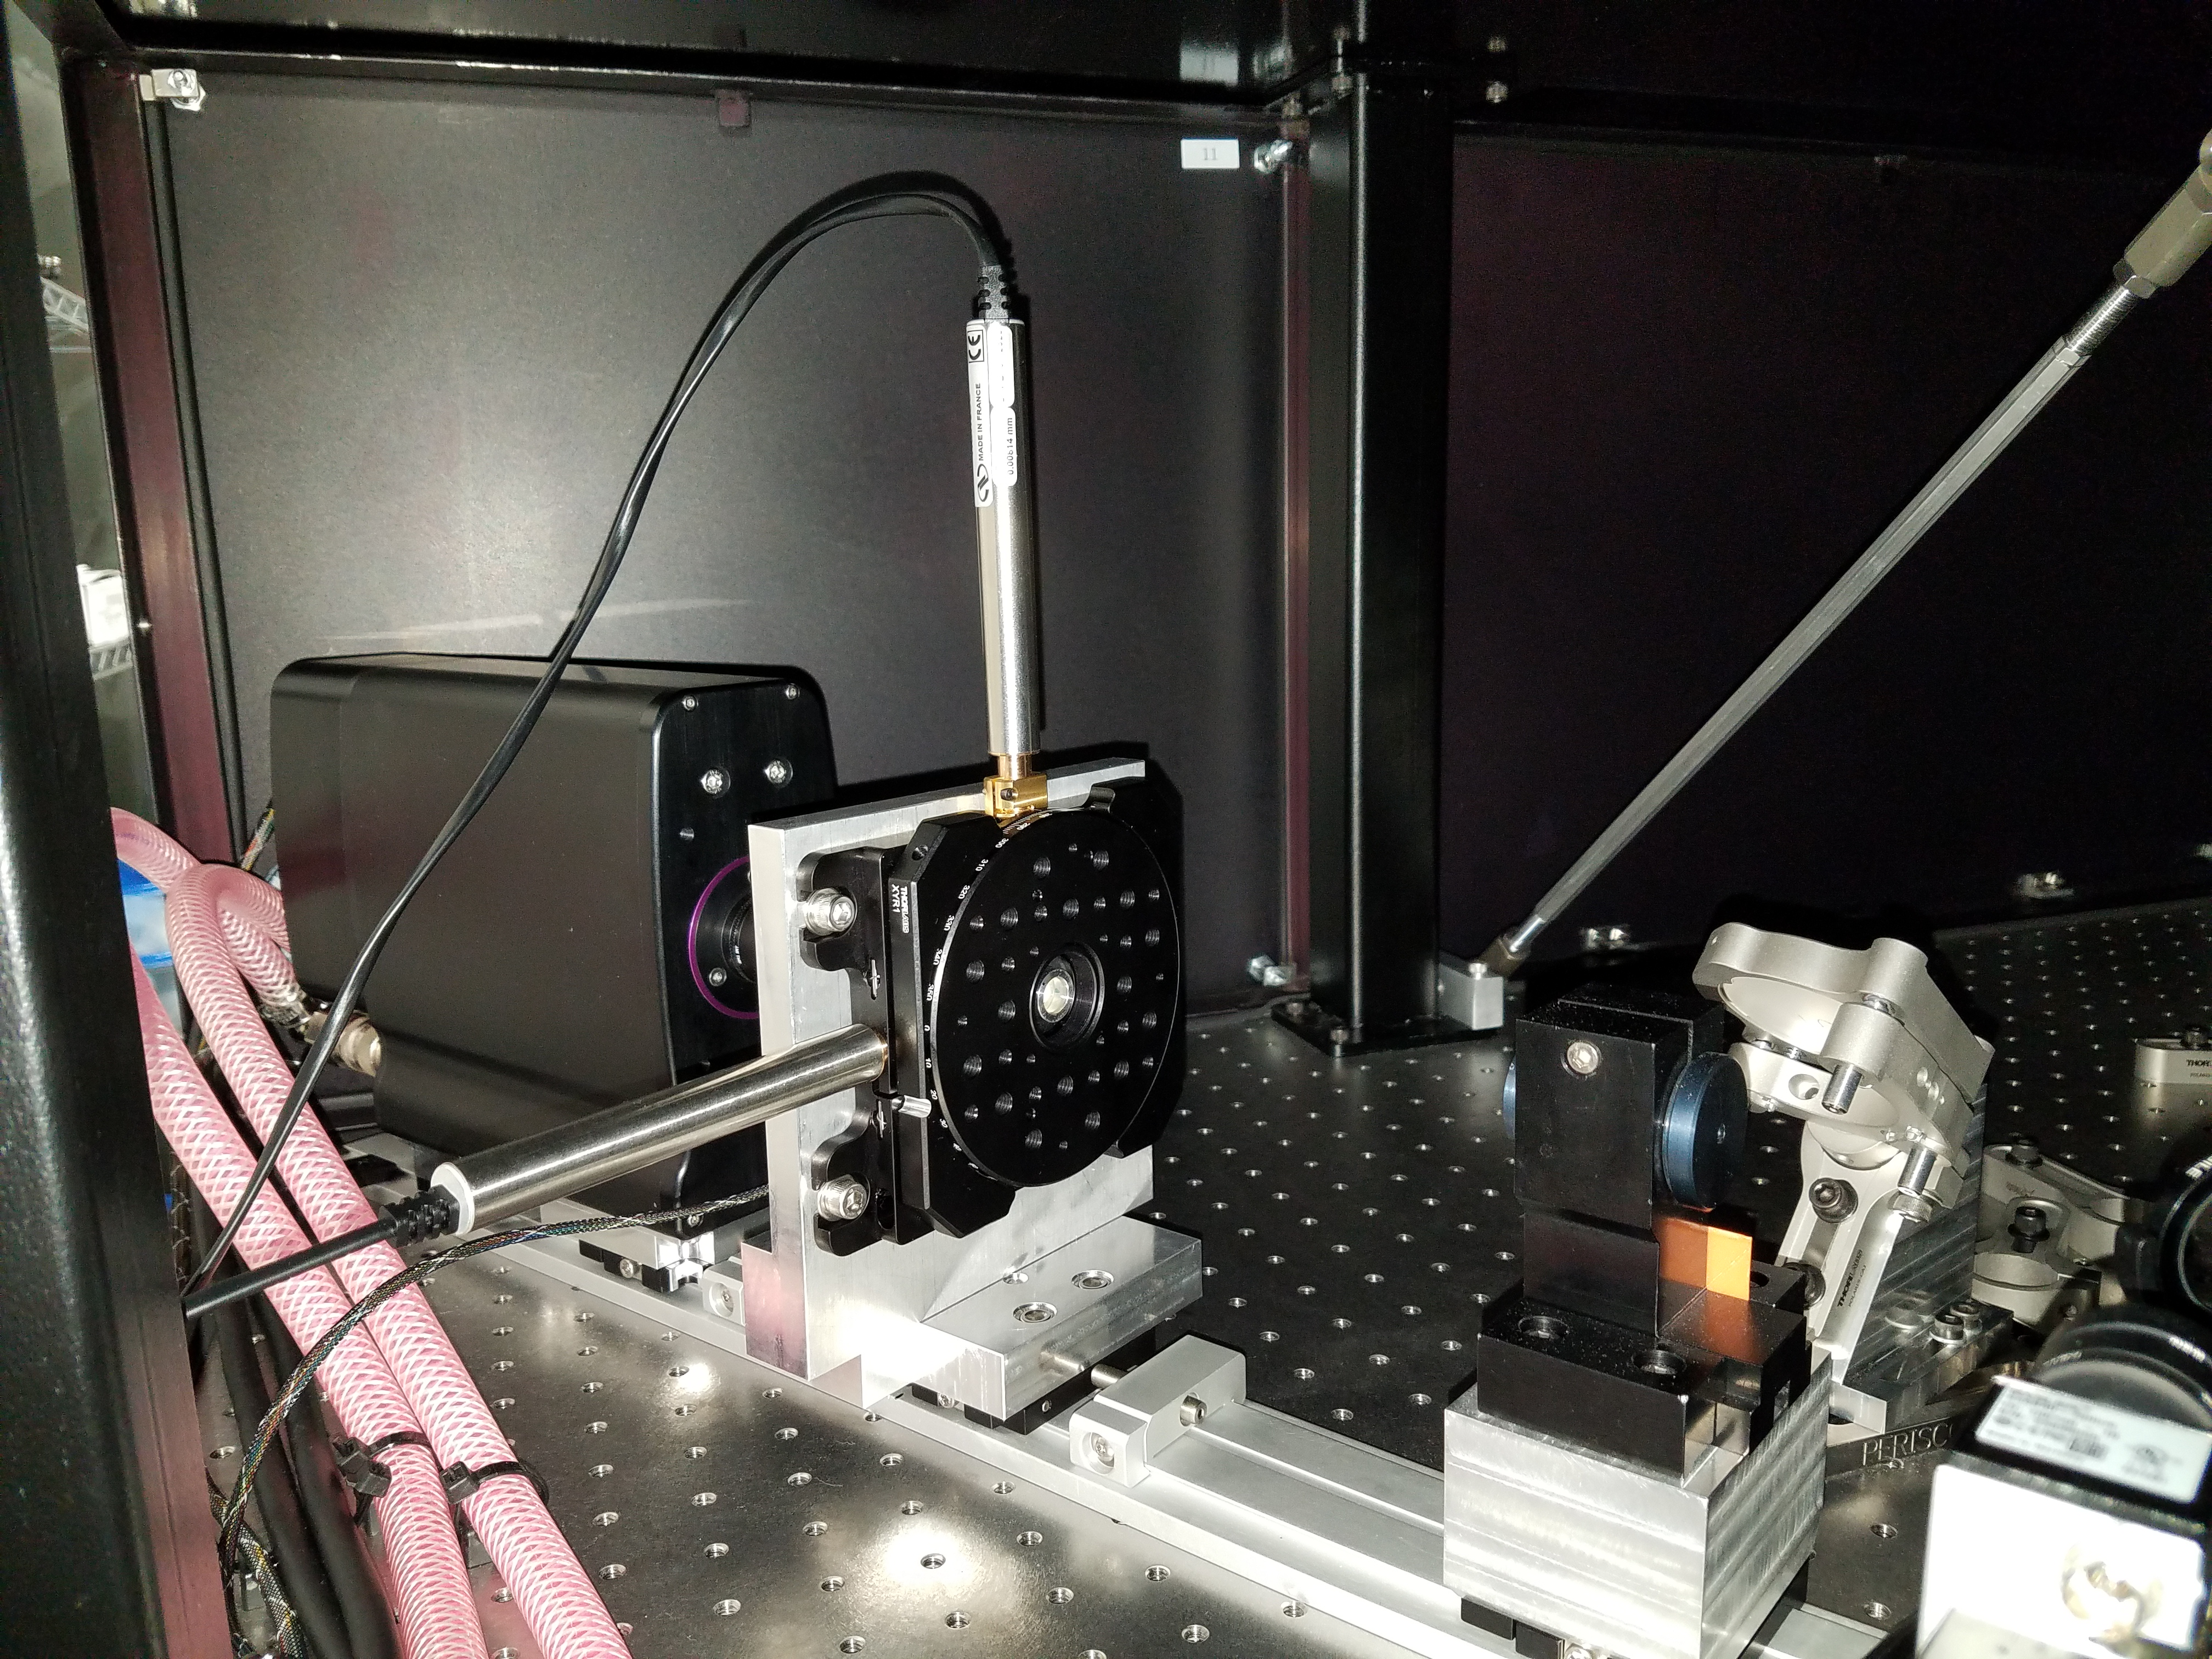
\includegraphics[width=.8\textwidth]{Chapter Materials/Chapter Three Materials/cameraLensPiezoHolder.png}
    \caption{The custom achromatic triplet lens mounted in a precision X-Y lens mount.}
    \label{fig:mountedtriplet}
\end{figure}
	
An initial alignment of the MagAO-X pyramid wavefront sensor was done using a HeNe single mode fiber laser, two off axis parabolic mirrors, and a temporary pupil mask with coarse edges. The pyramid optic, camera lens, and OCAM$^2$K were mounted on a coaxial rail system from ThorLabs as shown in Figure \ref{fig:mountedPWFS}. Custom mounting plates were fabricated for each optic, so that each could be mounted onto rail carriages and meet the beam height requirement of 5 inches from the optical table. 

\begin{figure}
    \centering
    \includegraphics[width=.8\textwidth]{Chapter Materials/Chapter Three Materials/mountedPWFS.jpg}
    \caption{The mounted pyramid optics, camera lens, and OCAM$^2$K camera on a coaxial rail from ThorLabs.}
    \label{fig:mountedPWFS}
\end{figure}

The mount of the pyramid optic has a custom target that aligns with the pyramid tip. To align the PWFS we first mounted the pyramid optic with the target on the optical rail and placed it on the MagAO-X optical table. The position of the rail and the tip/tilt of the incoming beam from OAP $\#5$, was adjusted iteratively until the beam hit the center of the target when the pyramid was placed at both the front and the back of the rail. This established the beam line for the system. The camera lens and OCAM$^2$K was then placed on the rail according to the Zemax design. The fine focus of the pyramid optic was dialed using a micrometer nudger, and by examining the signal of the pyramid pupils with and without modulation. The spacing of the camera lens and the OCAM$^2$ were adjusted until the size and separation of the pupils were in specifications. The measurement of the pupil parameters was done by a circle fit of the modulated pyramid pupils shown in Figure \ref{fig:fitPupils}. The average size of the MagAO-X pupils is 55.83 pixels in diameter. Figure \ref{fig:MagAOXpupils} shows the white light pupils of the MagAO-X PWFS under 5 $lambda/D$ modulation.

\begin{figure}
    \centering
    \includegraphics[width=.8\textwidth]{Chapter Materials/Chapter Three Materials/Age 170.668.jpeg}
    \caption{Caption}
    \label{fig:fitPupils}
\end{figure}

\begin{figure}
    \centering
    \includegraphics{Chapter Materials/Chapter Three Materials/MagAOXpupil5LD.png}
    \caption{The MagAO-X pyramid wavefront sensor pupils with 5 $\lambda/D$ modulation. The spiders and central obscuration are from the aperture of the Magellan Telescope.  }
    \label{fig:MagAOXpupils}
\end{figure}